\documentclass[121pt, aspectratio=169, t]{beamer}
\usepackage[utf8]{inputenc}
\usepackage[brazil]{babel}
\usepackage{beamerthemesplit}

%-----------------------------------------------------------------------------------------------
% --- Slide Justificado --------------------------------------------------------------
\usepackage{ragged2e}
\usepackage{etoolbox}
\usepackage{soul}
\usepackage[normalem]{ulem}
\usepackage{cancel}
\usepackage{bm}
\usepackage{array}
\usepackage{wrapfig} 
\apptocmd{\frame}{}{\justifying}{} % Allow optional arguments after frame.
\usepackage{amsmath,mathtools}
\usepackage{scrextend} % ajustar texto para direita
%\usepackage{enumitem}
%\usepackage{showframe}
% =============================================================================
% Pacotes para simbolos IPA
% =============================================================================
\usepackage{tipa}		% Simbolos do IPA
\usepackage{tipx}
%-----------------------------------------------------------------------------------------------
% separação entre colunas e linhas de tabelas
\setlength{\tabcolsep}{2pt}
\renewcommand{\arraystretch}{1}
%-----------------------------------------------------------------------------------------------
% Define a centralização de coluna com largura {|C{1 cm}|}
\newcolumntype{C}[1]{>{\centering\let\newline\\\arraybackslash\hspace{0pt}}m{#1}}
\newcolumntype{L}[1]{>{\raggedright\let\newline\\\arraybackslash\hspace{0pt}}m{#1}}
%-----------------------------------------------------------------------------------------------
\newcommand\litem[1]{\item{\bfseries #1 }}
% --- Configuracoes de Tema e cores --------------------------------------------------
\usetheme{CambridgeUS}

\definecolor{darkblue}{rgb}{0.07058,0.06470,0.01176}  % Preto 		RGB 21,20,16
\definecolor{yellow}{rgb}{0.57058,0.66470,0.71176} 	
\definecolor{myred}{rgb}{0.808,0.086,0.133}   % 0.98823,0.00000,0.00784
% amarelo	RGB (1,1,0.588224) 255,255,150 PAULA 4
\definecolor{myblue}{rgb}{0.57058,0.66470,0.71176} % azul 	RGB 13,29,174

\setbeamercolor{item}{fg=myblue}

\setbeamercolor{alerted text}{fg=yellow}	
\setbeamercolor*{palette primary}{fg=darkblue,bg=yellow}
\setbeamercolor*{palette secondary}{fg=darkblue,bg=myred}
\setbeamercolor*{palette tertiary}{bg=darkblue,fg=yellow}
\setbeamercolor*{palette quaternary}{fg=darkblue,bg=yellow}

\setbeamercolor*{sidebar}{fg=darkblue,bg=orange!75!white}

\setbeamercolor*{palette sidebar primary}{fg=darkblue}
\setbeamercolor*{palette sidebar secondary}{fg=white}
\setbeamercolor*{palette sidebar tertiary}{fg=white} % darkblue!50!black
\setbeamercolor*{palette sidebar quaternary}{fg=white} % yellow!10!orange

\setbeamercolor*{titlelike}{parent=palette primary}
\setbeamercolor{frametitle}{bg=yellow}
\setbeamercolor{frametitle right}{bg=yellow}

\setbeamercolor*{separation line}{bg=myblue}
\setbeamercolor*{fine separation line}{bg=myblue}


% --- Letras e simbolos matemáticos --------------------------------------------------
% ------------------------------------------------------------------------------------
\usepackage[bbgreekl]{mathbbol}  % Pacote para repreentação de conjuntos com \mathbb{R} com letras gregas
\usepackage{amsfonts}	% Pacote para repreentação de conjuntos com \mathbb{R}
\usepackage{mathrsfs}	% Pacote para letras matemáticas

\usepackage{amssymb} 	% diversos simbolos matematicos adicionais. Carrega automático com amsfonts
% ------------------------------------------------------------------------------------
\usepackage{multicol}

\usepackage{multimedia}
\usepackage[]{graphicx}
\usepackage[]{color}
\usepackage{geometry}
\usepackage{media9}

\usepackage{tabularx}
\usepackage{amsmath, amsthm, amssymb}
\usepackage{gensymb}

% ------------------------------------------------------------------------------------

% --- Esta definicao deve vir antes --------------------------------------------------
\usepackage{graphicx}			% Inclusão de gráficos
\usepackage{float}  
% ------------------------------------------------------------------------------------
\usefonttheme[onlymath]{serif}
\usepackage{hyperref}
\usepackage{multirow}
\usepackage{subfig}
\usepackage{ragged2e}
\captionsetup[subfigure]{labelformat=empty}
\usepackage{color}
\usepackage{colortbl}
\usepackage{textpos}
\usepackage{tikz}
\usetikzlibrary{calc}
%---------------
\usepackage{tabularx}
\usepackage{booktabs}

\usepackage{multimedia}

%\newenvironment{leftbox}[1]
%{\itemize[
%	nosep,
%	leftmargin=0pt,
%	rightmargin=\dimexpr\textwidth-#1\relax,
%	itemindent=\parindent,
%	listparindent=\parindent,
%	]\item[]\relax}
%{\enditemize}
%
%\newenvironment{rightbox}[1]
%{\itemize[
%	nosep,
%	leftmargin=\dimexpr\textwidth-#1\relax,
%	rightmargin=0pt,
%	itemindent=\parindent,
%	listparindent=\parindent,
%	]\item[]\relax}
%{\enditemize}

\def\DISCIPLINA/{Introdução à Linguística Computacional: Linguística de Corpus, Processamento de Linguagem Natural e Aplicações}
\def\DISC/{Introdução à Linguística Computacional}

\tikzset{
	invisible/.style={opacity=0},
	visible on/.style={alt={#1{}{invisible}}},
	alt/.code args={<#1>#2#3}{%
		\alt<#1>{\pgfkeysalso{#2}}{\pgfkeysalso{#3}} % \pgfkeysalso doesn't change the path
	},
}

\newenvironment{caixadireita}[2][.5\linewidth]
{\par\hfill\tabular{@{}p{#1}@{}}
	\multicolumn{1}{@{}c@{}}{#2} \\ }
{\endtabular\par}

% --- Desativando os botoes de navegacao ---------------------------------------------
\setbeamertemplate{navigation symbols}{}
% ------------------------------------------------------------------------------------
% --- Tela cheia ---------------------------------------------------------------------
\hypersetup{pdfpagemode=FullScreen}
% ------------------------------------------------------------------------------------
% --- Layout da pagina ---------------------------------------------------------------
\hypersetup{pdfpagelayout=SinglePage}
% ------------------------------------------------------------------------------------
% --- Relaxed footnotes --------------------------------------------------------------
\newcommand{\lfr}[1]{\let\thefootnote\relax\footnote{\tiny #1}}
% --- Pasta com as imagens -----------------------------------------------------------
\graphicspath{{Imagens/}}
\DeclareMathOperator{\erf}{erf}
% ------------------------------------------------------------------------------------
\title[Linguística Computacional]{Introdução ao Processamento de Voz e Fala}
\author[Silva, A. P.]{Adelino Pinheiro Silva\vspace{0cm}}
\institute[ADA]{ \footnotesize{Universidade Federal de Minas Gerais (UFMG) \\ Faculade de Letras (FALE) \\ \DISC/ } \\ \vspace{0cm}}
\date{\today}

\begin{document}
	\begin{tikzpicture}[remember picture,overlay]
		\node[xshift=-4.5cm,yshift=-3.25cm,opacity=1.0] at (current page.center) {
\includegraphics[width=6cm]{ADA_logo-borda.png}};
	\end{tikzpicture}
	\frame{\titlepage}
% ==============================================================================
% TEMPLATE - frame com imagem
%\begin{frame}[fragile=singleslide]
%	\frametitle{Visão Geral das Ciências Forenses}
%	\begin{tikzpicture}[remember picture,overlay]
%		\node[xshift=0cm,yshift=-0.5cm,opacity=1.0] at (current page.center) {\includegraphics[width=13cm]{Diagrama_Historia_Forense.pdf}};
%	\end{tikzpicture}
%	\vfill
%	\lfr{Imagem: {Arquivo do autor.}}
%\end{frame}
% TEMPLATE - frame com tópicos e imagens
%\begin{frame}[fragile=singleslide]
%	\frametitle{Visão Geral das Ciências Forenses}
%	\begin{itemize}[]
%		\item Conjunto de conhecimentos e técnicas.
%		\item Aplicadas a assuntos legais.
%		\item Livro Xi Yuan Lu (Registro de injustiça \\ ou lavagem dos erros).
%		\item Escola alemã \textit{Kriminalistik}.
%		\item Escola Francesa Locard.
%		%		\item 
%	\end{itemize}
%	\vspace{0.75cm}
%	\begin{itemize}[]
%		\item Arquimedes, Poincaré, 
%		\item Conan Doyle, Maurice Leblanc, Barry Allen.
%	\end{itemize}
%	
%	\begin{tikzpicture}[remember picture,overlay]
%		\node[xshift=4.75cm,yshift=0.5cm,opacity=1.0] at (current page.center) {\includegraphics[width=6cm]{Foto-Henrique-Almeida-11.jpg}};
%	\end{tikzpicture}
%	\vfill
%	\lfr{Imagem: \url{https://noticias.paginas.ufsc.br/files/2022/09/Foto-Henrique-Almeida-11.jpg}}
%	
%\end{frame}


% ==============================================================================
	
% ==== Sumário =================================================================
\section{Sumário}
\begin{frame}
	\frametitle{Sumário}
	\tableofcontents
\end{frame}
% ==============================================================================

% ==============================================================================
\AtBeginSection[]
{
	\begin{frame}
		\frametitle{Assuntos}
		\tableofcontents[currentsection]
	\end{frame}
}
% ==============================================================================
\section{Aplicações}
% ------------------------------------------------------------------------------
\begin{frame}
\frametitle{Acessibilidade, Inclusão e Educação}
	\begin{itemize}[]
		\item Interface homem máquina.
		\item Tradução e interpretação.
		\item Conversão de texto para voz e voz para texto.
		\item Assistentes inteligentes.
	\end{itemize}
	\begin{tikzpicture}[remember picture,overlay]
			\node[xshift=2.75cm,yshift=-1.5cm,opacity=1.0] at (current page.center) {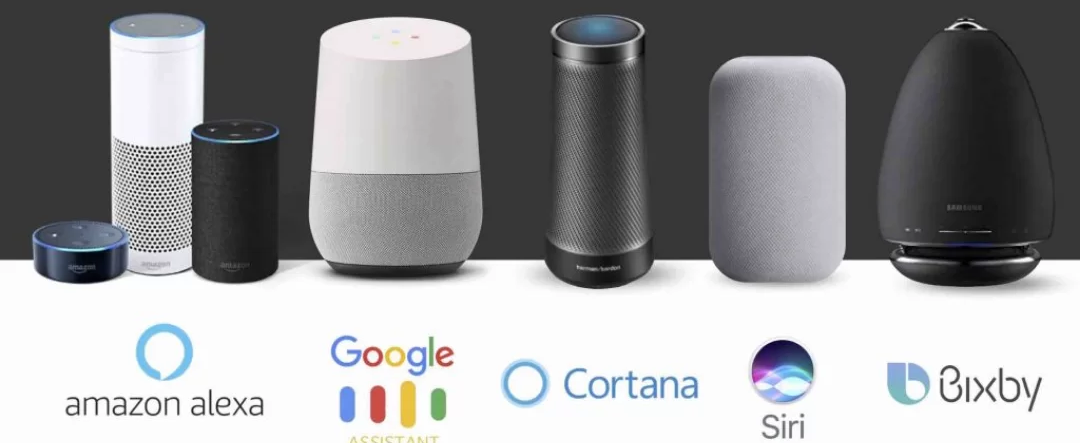
\includegraphics[width=10cm]{assistentes.png}};
	\end{tikzpicture}
	\vfill
	\lfr{Imagem: \url{https://eletronjun.com.br/wp-content/uploads/2021/03/image1-1-edited.png}}
\end{frame}
% ------------------------------------------------------------------------------
\begin{frame}
\frametitle{Comunicação, Saúde e Segurança}
	\begin{itemize}[]
		\item Comunicação a distância.
		\item Triagem e diagnóstico de distúrbios da voz.
		\item Avaliação de fluência.
		\item Biometria.
		\item Comparação Forense de Locutor.
	\end{itemize}
	\begin{tikzpicture}[remember picture,overlay]
		\node[xshift=3.25cm,yshift=-1.5cm,opacity=1.0] at (current page.center) {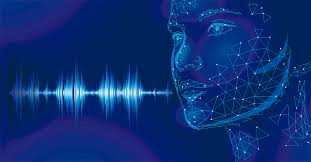
\includegraphics[width=8cm]{biometria.jpeg}};
	\end{tikzpicture}
	\vfill
	\lfr{Imagem: \url{https://encrypted-tbn0.gstatic.com/images}}
\end{frame}
% ------------------------------------------------------------------------------
\begin{frame}
\frametitle{Natureza, Entretenimento, Mimetização}
	\begin{itemize}[]
		\item Reconhecimento de espécies.
		\item Psicoacústica.
		\item Autotune.
		\item \textit{Deep fakes}.
		\item Dublagem automática.
	\end{itemize}
	\begin{tikzpicture}[remember picture,overlay]
		\node[xshift=3.25cm,yshift=-1.0cm,opacity=1.0] at (current page.center) {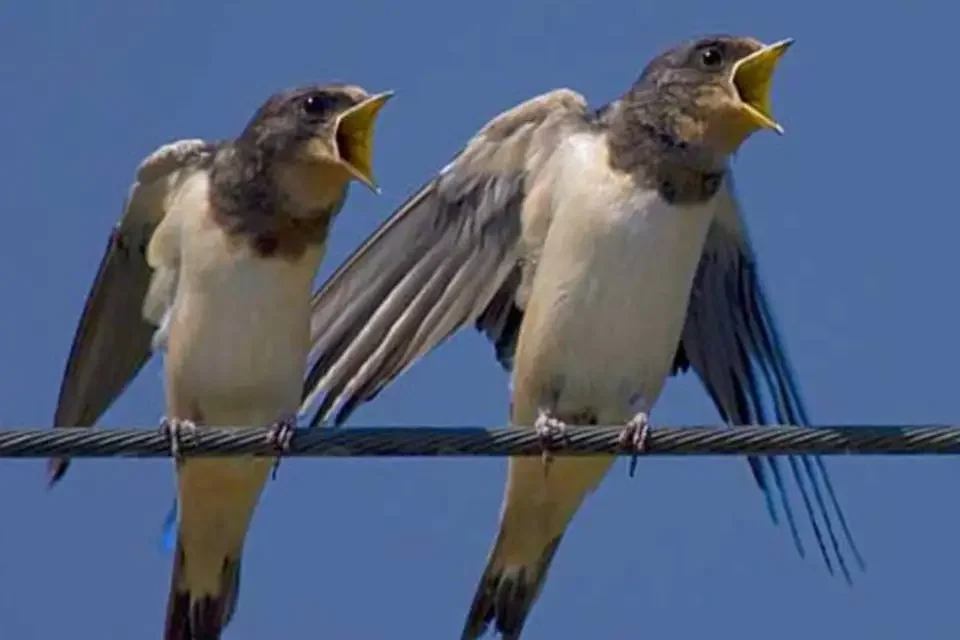
\includegraphics[width=7cm]{identifica_passaros.png}};
	\end{tikzpicture}
	\vfill
	\lfr{Imagem: \url{https://classic.exame.com/wp-content/uploads/2016/09/size_960_16_9_twitter-passaros1.jpg}}
\end{frame}
% ------------------------------------------------------------------------------
% ==============================================================================
\section{Representação digital do som}
\begin{frame}
	\frametitle{Sinal da voz e da fala}
	\large{Onda acústica: onda de pressão longitudinal por compressão e descompressão.}
	\begin{itemize}[]
		\item Amplitude.
		\item Frequência.
		\item Fase.
	\end{itemize}	
	
	\begin{tikzpicture}[remember picture,overlay]
		\node[xshift=1.25cm,yshift=-1.0cm,opacity=1.0] at (current page.center) {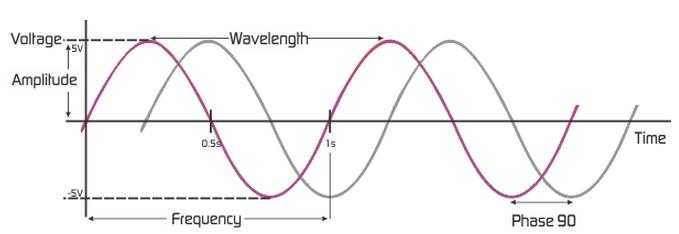
\includegraphics[width=12cm]{amplitude-frequency-wavelenght-phase.jpg}};
	\end{tikzpicture}
	\vfill
	\lfr{Imagem: \url{https://fiberbit.com.tw/wp-content/uploads/2013/07/}}
\end{frame}
% ------------------------------------------------------------------------------
\begin{frame}
	\frametitle{Da natureza para o computador}

	\large{No quadro...}

	\begin{itemize}[]
		\item Amostragem \\ taxa de amostragem e limitação de banda.
		\item Quantização  \\ ruído $SNR(dB) = 6B -7,2 dB$.
		\item Número de canais \\ \textit{mono}, \textit{stereo}, 5.1 ...
		\item Armazenamento  \\ tamanho do arquivo WAV PCI.
	\end{itemize}

	\begin{tikzpicture}[remember picture,overlay]
		\node[xshift=4.25cm,yshift=-0.5cm,opacity=1.0] at (current page.center) {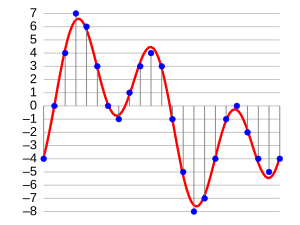
\includegraphics[width=8cm]{4-bit-linear-PCM.svg.png}};
	\end{tikzpicture}
	\vfill
	\lfr{Imagem: \url{https://upload.wikimedia.org/wikipedia/commons/thumb/2/21/4-bit-linear-PCM.svg}}

\end{frame}
% ==============================================================================
\section{Análise em frequência}
\begin{frame}
	\frametitle{Definição para \textbf{ondas periódicas}}
	\large{Decomposição de uma onda ``complexa'' em um conjunto de ondas simples.}
	
	\begin{tikzpicture}[remember picture,overlay]
		\node[xshift=0cm,yshift=-1.0cm,opacity=1.0] at (current page.center) {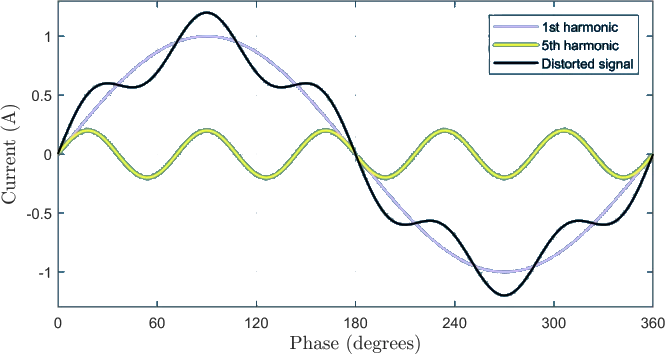
\includegraphics[width=10cm]{Fifth-Harmonic-waveform-1-768x384.png}};
	\end{tikzpicture}
	\vfill
	\lfr{Imagem: \url{https://power-converters.net/wp-content/uploads/2022/03/}}
	
\end{frame}
% ------------------------------------------------------------------------------
\begin{frame}
	\frametitle{A partir de uma frequência fundamental...}
	\large{Múltiplos inteiros com mudança de amplitude e fase}
	
	\begin{tikzpicture}[remember picture,overlay]
		\node[xshift=0cm,yshift=-0.75cm,opacity=1.0] at (current page.center) {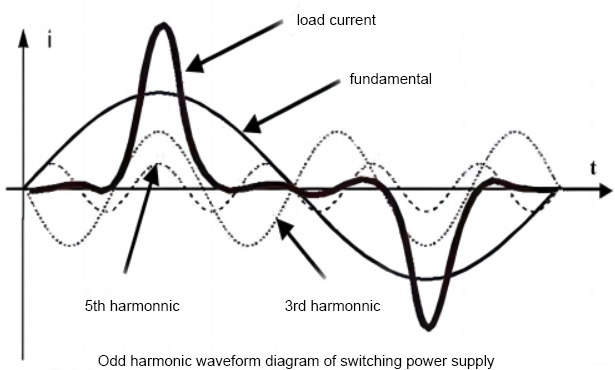
\includegraphics[width=9cm]{20240530113826_26978.png}};
	\end{tikzpicture}
	\vfill
	\lfr{Imagem: \url{https://www.zddqelectric.com/js/htmledit/kindeditor/attached/20240530/}}
	
\end{frame}
% ------------------------------------------------------------------------------
\begin{frame}
	\frametitle{Ferramentas matemáticas}
	
	\begin{tikzpicture}[remember picture,overlay]
		\node[xshift=1cm,yshift=-0.5cm,opacity=1.0] at (current page.center) {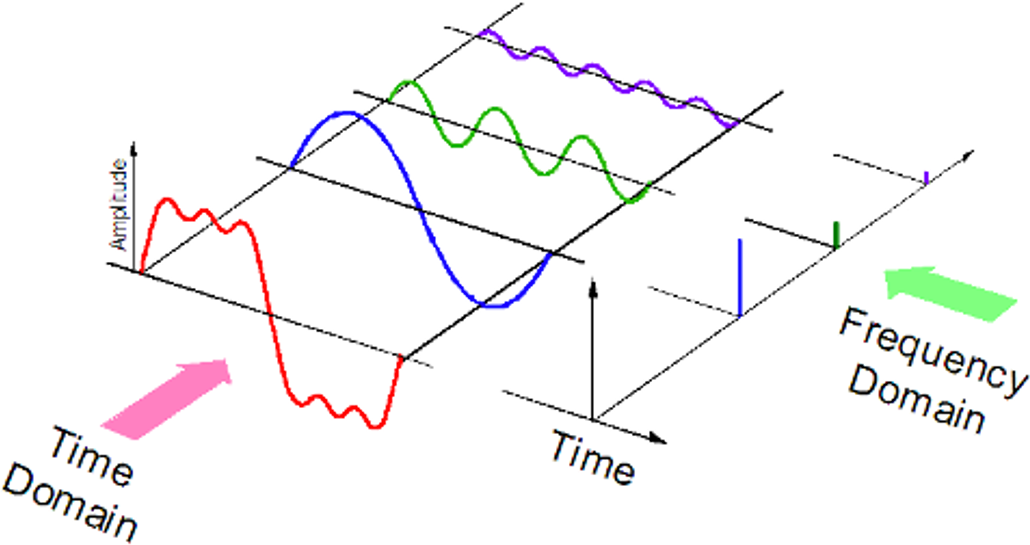
\includegraphics[width=12cm]{fft_01.png}};
	\end{tikzpicture}
	\large{FFT (\textit{fast Fourier transform})}
	\vfill
	\lfr{Imagem: \url{https://miro.medium.com/v2/resize:fit:1358/1*w1mcpi8gCgQI4FrqWFJ2GA.png}}
	
\end{frame}
% ------------------------------------------------------------------------------
\begin{frame}
	\frametitle{FFT (\textit{fast Fourier transform})}
	\begin{tikzpicture}[remember picture,overlay]
		\node[xshift=1cm,yshift=-0.5cm,opacity=1.0] at (current page.center) {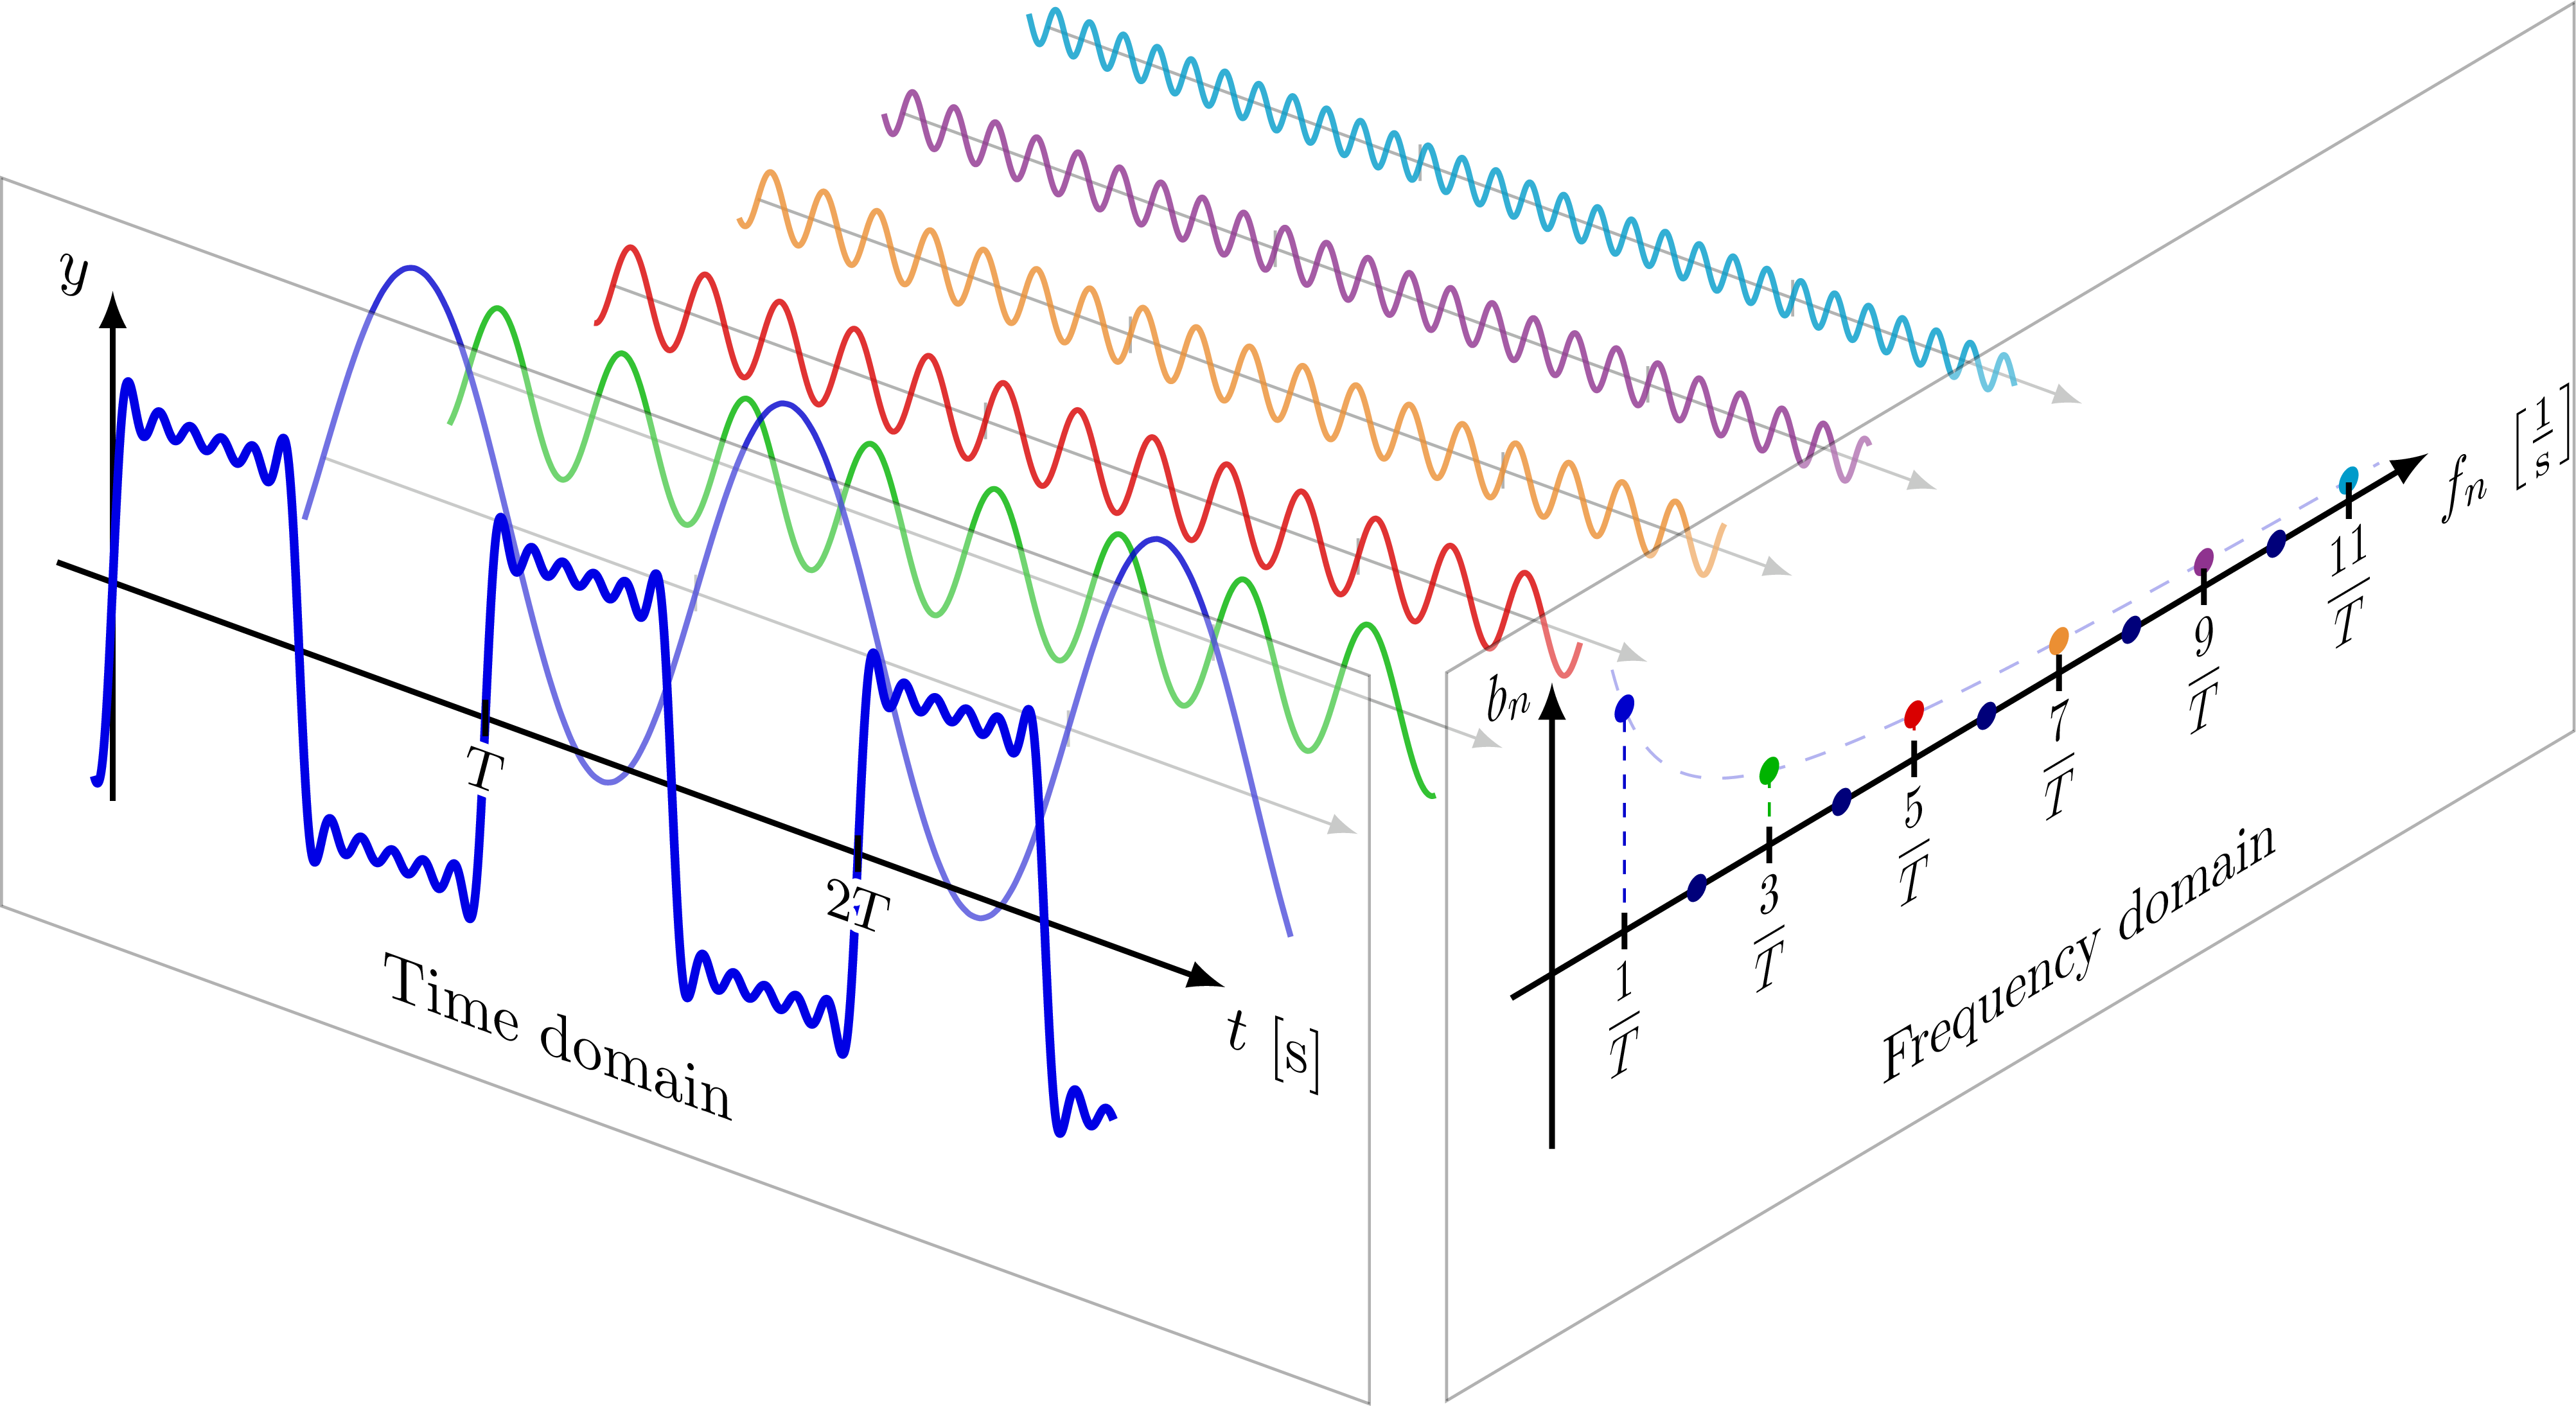
\includegraphics[width=13cm]{fourier_series-011.png}};
	\end{tikzpicture}
	\vfill
	\lfr{Imagem: \url{https://tikz.net/files/}}
	
\end{frame}
% ------------------------------------------------------------------------------
\begin{frame}
	\frametitle{Espectrograma}
	\begin{tikzpicture}[remember picture,overlay]
		\node[xshift=1cm,yshift=-0.75cm,opacity=1.0] at (current page.center) {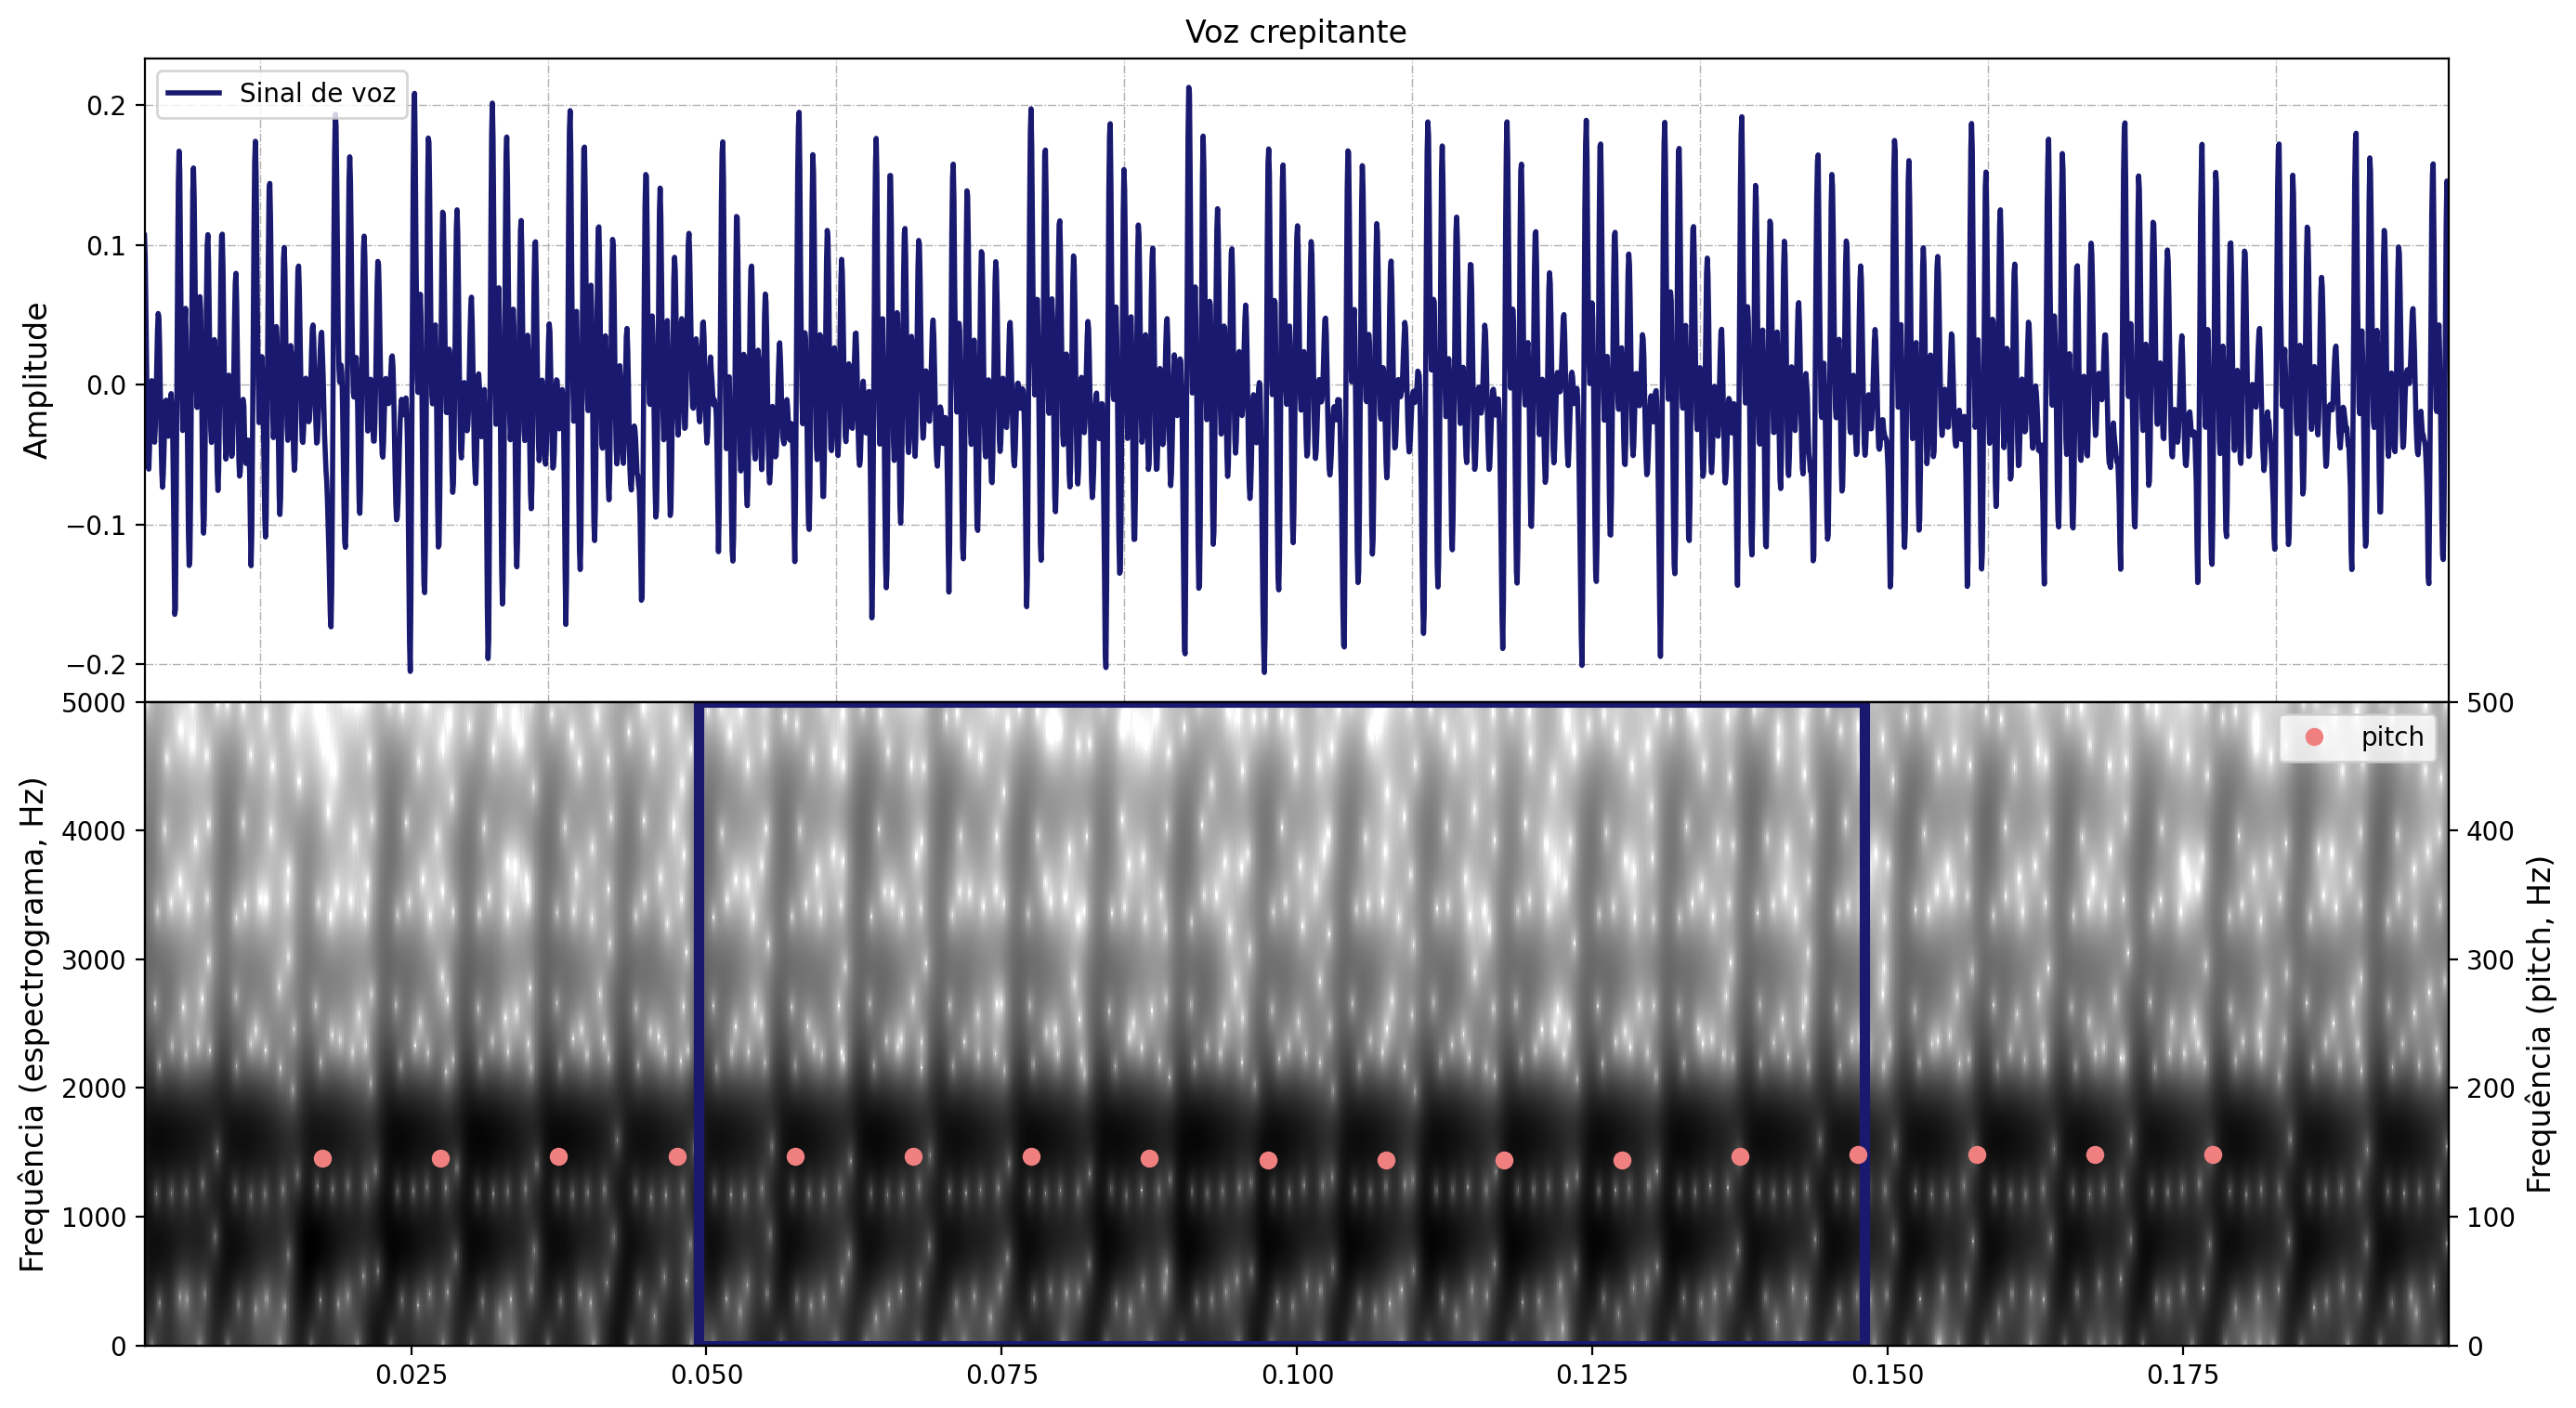
\includegraphics[width=11cm]{F011_crepitante.png}};
	\end{tikzpicture}
	\large{FFT de pequenos pedacinhos do áudio}
	\vfill
	\lfr{Imagem: \url{http://www.poslin.letras.ufmg.br/diss_defesas_detalhes.php?aluno=2312}}	
		
\end{frame}
% ------------------------------------------------------------------------------
\begin{frame}
	\frametitle{Espectrograma... No quadro}
	\begin{tikzpicture}[remember picture,overlay]
		\node[xshift=1cm,yshift=-0.75cm,opacity=1.0] at (current page.center) {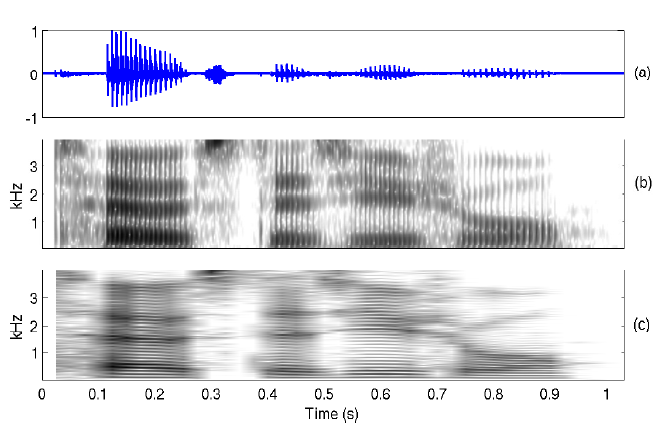
\includegraphics[width=10cm]{wbnb.png}};
	\end{tikzpicture}
	\large{Relação de compromisso entre tempo e frequência}
	\vfill
	\lfr{Imagem: \url{https://ssp-iiith.vlabs.ac.in/exp/spectrographic-analysis/}}	
		
\end{frame}
% ==============================================================================
\section{Medições no sinal de voz e fala}
\begin{frame}
	\frametitle{Começando do básico}
		\begin{itemize}[]
			\item Duração.
			\item Intensidade.
			\item Frequência fundamental.
			\item Formantes.
		\end{itemize}	
		\begin{tikzpicture}[remember picture,overlay]
			\node[xshift=2.25cm,yshift=-0.5cm,opacity=1.0] at (current page.center) {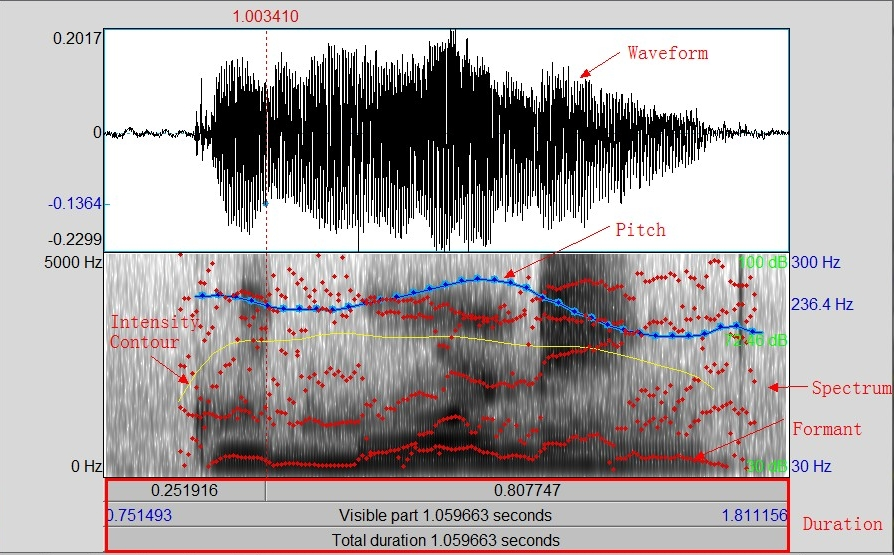
\includegraphics[width=10cm]{Praat1.49.jpg}};
		\end{tikzpicture}
		\vfill
		\lfr{Imagem: \url{https://corpus.eduhk.hk/english_pronunciation/wp-content/uploads/2020/03/}}
	
\end{frame}
% ------------------------------------------------------------------------------ 
\begin{frame}
	\frametitle{Duração}
	\begin{tikzpicture}[remember picture,overlay]
		\node[xshift=3cm,yshift=0.0cm,opacity=1.0] at (current page.center) {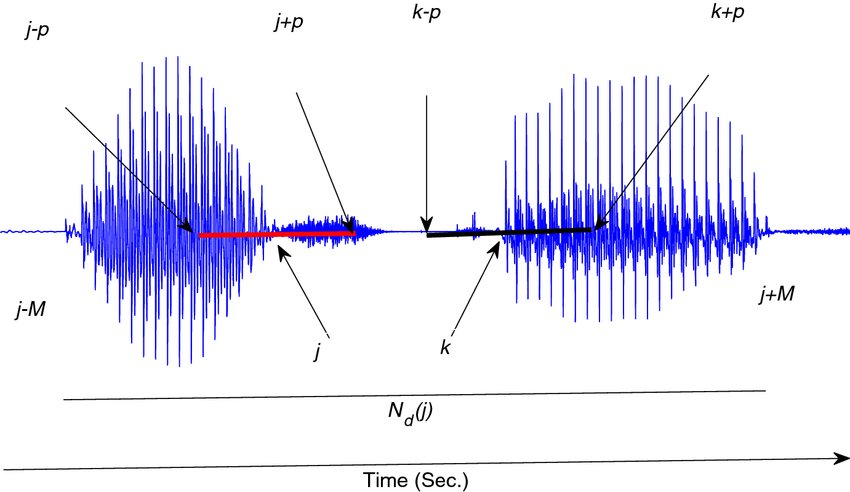
\includegraphics[width=9cm]{Illustration-of-NLM.png}};
	\end{tikzpicture}
	\vspace{-0.5cm}
	\begin{large}
		\begin{itemize}[]
			\item Como é medido:
			\begin{itemize}[]
				\item Intervalo entre início e fim.
			\end{itemize}	
			\item Para que serve:
			\begin{itemize}[]
				\item Localização de acentos.
				\item Interpretação de contexto.
				\item Fluência de leitura.
			\end{itemize}	
		\end{itemize}	
	\end{large}
	\vfill
	\lfr{Imagem: \url{https://www.researchgate.net/publication/330973772}}
\end{frame}
% ------------------------------------------------------------------------------ 
\begin{frame}
	\frametitle{Intensidade}
	\begin{tikzpicture}[remember picture,overlay]
		\node[xshift=3cm,yshift=0.0cm,opacity=1.0] at (current page.center) {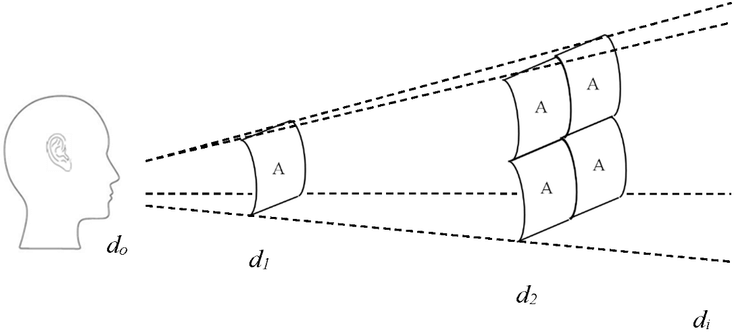
\includegraphics[width=9cm]{Sound-intensity.png}};
	\end{tikzpicture}
	\vspace{-0.5cm}
	\begin{large}
		\begin{itemize}[]
			\item Como é medido:
			\begin{itemize}[]
				\item Na onda: valor da raiz quadrada média.
				\item SPL: razão logarítmica.
			\end{itemize}	
			\item Para que serve:
			\begin{itemize}[]
				\item Localização de acentos.
				\item Capacidade de fala.
				\item Distúrbios respiratórios.
			\end{itemize}	
		\end{itemize}
	\end{large}
		
	\vspace{1cm}
	\hspace{1cm} $SPL(dB) = 10 \log_{10} \left(\frac{P_{med}}{p_0} \right)^2$
	
	\hspace{1cm} $p_0 = 20~\mu Pa$
	
	
	\vfill
	\lfr{Imagem: \url{https://www.researchgate.net/publication/336227251/}}
	
\end{frame}
% ------------------------------------------------------------------------------ 
\begin{frame}
	\frametitle{Frequência fundamental}
	
	\begin{large}
		\begin{itemize}[]
			\item Como é medido:
			\begin{itemize}[]
				\item Correlação.
				\item Espetrograma.
			\end{itemize}	
			\item Para que serve:
			\begin{itemize}[]
				\item Estado emocional.
				\item Prosódia.
				\item Distúrbios da fala.
				\item Parâmetro biométrico.
			\end{itemize}	
		\end{itemize}	
	\end{large}
	\begin{tikzpicture}[remember picture,overlay]
		\node[xshift=3.5cm,yshift=-0.5cm,opacity=1.0] at (current page.center) {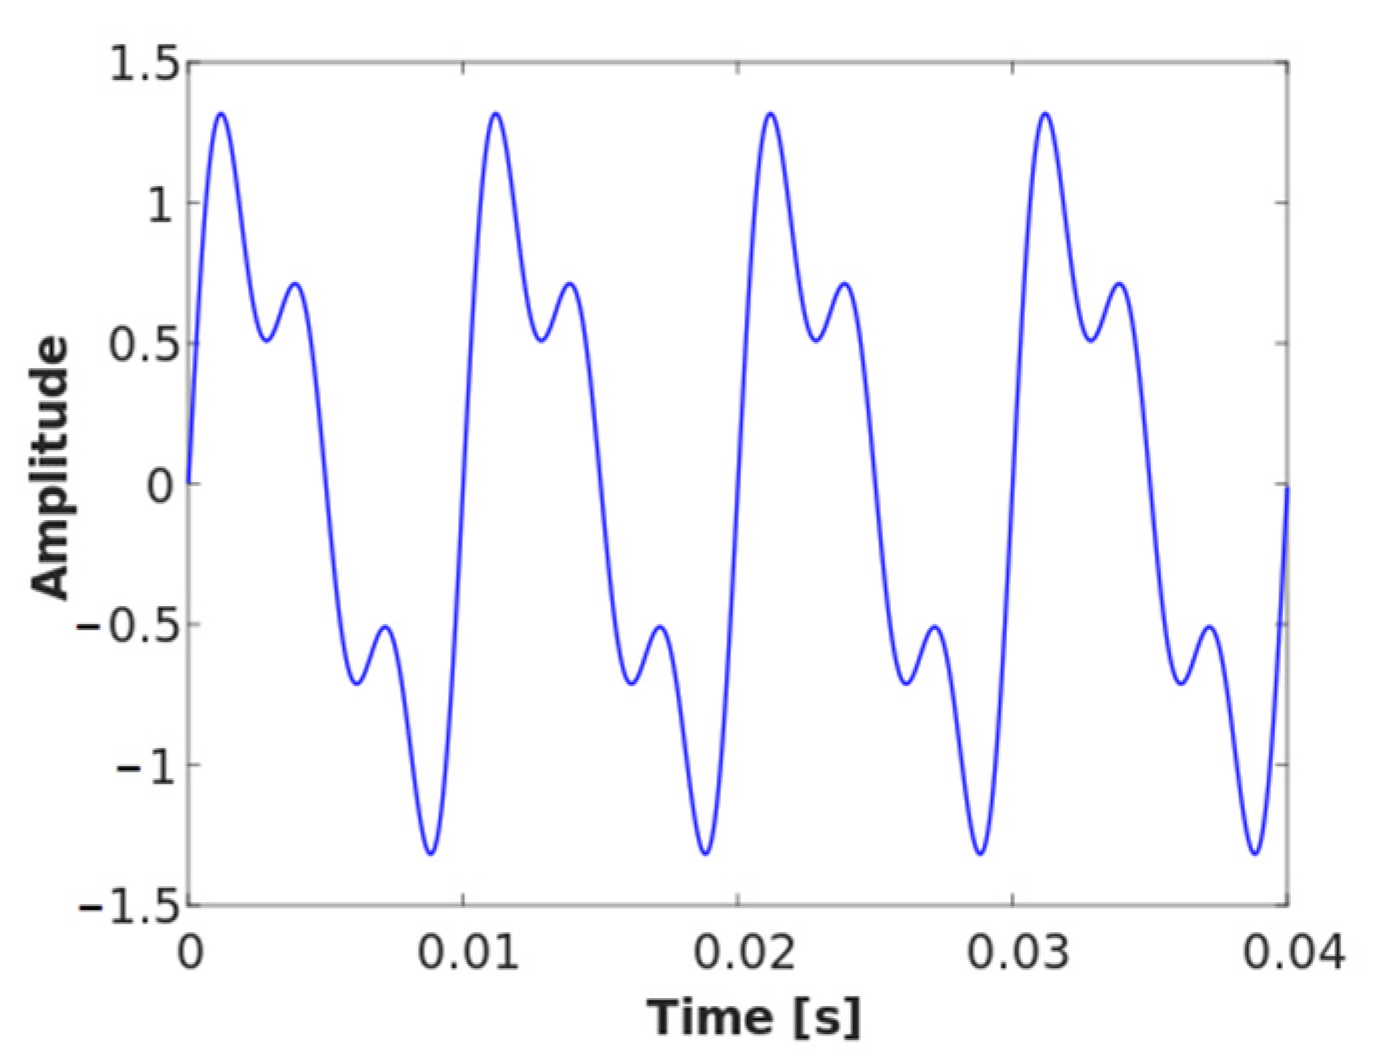
\includegraphics[width=8cm]{applsci-13-08191-g001.png}};
	\end{tikzpicture}
	\vfill
	\lfr{Imagem: \url{https://www.mdpi.com/applsci/applsci-13-08191}}
\end{frame}
% ------------------------------------------------------------------------------ 
\begin{frame}
	\frametitle{Formantes}
	\begin{large}
		\begin{itemize}[]
			\item Como é medido:
			\begin{itemize}[]
				\item FFT e análise LPC.
			\end{itemize}	
			\item Para que serve:
			\begin{itemize}[]
				\item Avaliação de fluência.
				\item Distúrbios da fala.
				\item Biometria.
				\item Identificação da fala.
			\end{itemize}	
		\end{itemize}
	\end{large}
	\begin{tikzpicture}[remember picture,overlay]
		\node[xshift=3.5cm,yshift=-0.5cm,opacity=1.0] at (current page.center) {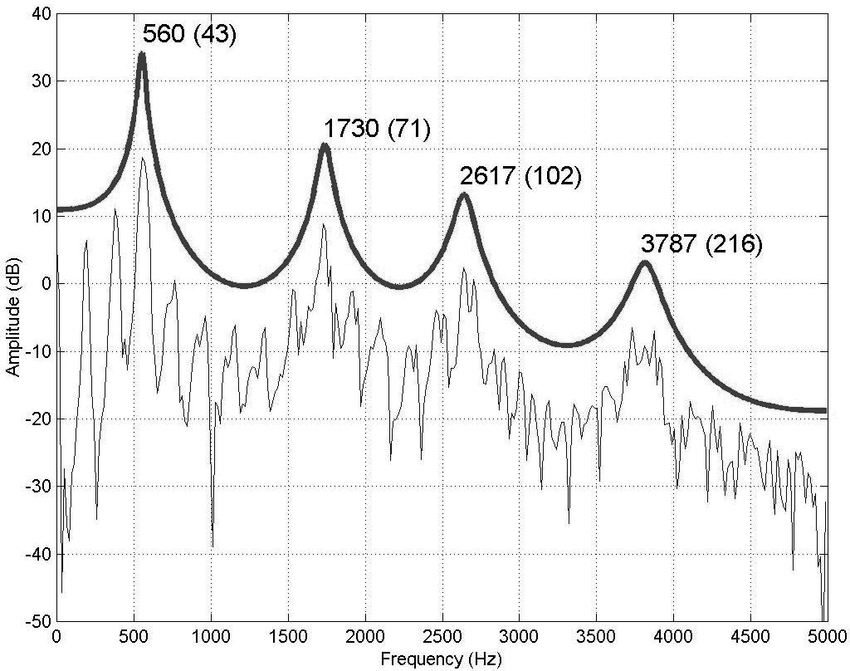
\includegraphics[width=8cm]{LPC-and-FFT-spectra.png}};
	\end{tikzpicture}
	\vfill
	\lfr{Imagem: \url{https://www.researchgate.net/profile/Phil-Rose/publication/274326216/}}

\end{frame}
% ------------------------------------------------------------------------------ 
% ------------------------------------------------------------------------
\section{Encerramento}
\begin{frame}[fragile=singleslide]
	\frametitle{Agradecimentos}
	
	\begin{center}
		\textbf{Fim!}
	\end{center}
	\vspace{-0.25cm}
	\begin{small}
		Contatos:
		\begin{itemize}
			\item e-mail: adelinocpp@gmail.com, adelinocpp@yahoo.com, adelino@ufmg.br ou adelino.pinheiro@policiacivil.mg.gov.br;
			\item  Whatsapp (31) 98801-3605;
			\item Instituto de Criminologia - Academia de Polícia Civil de Minas Gerais. Rua Oscar Negrão de Lima, 200, Nova Gameleira, Belo Horizonte-MG. Tel.: (31) 3314-5620;
			\item Setor de Perícias em Áudio e Vídeo - Instituto de Criminalística. Av. Augusto de Lima, 1833, Barro Preto, Belo Horizonte-MG. Tel.: (31) 3330-1887;
			
		\end{itemize}        
	\end{small}
\end{frame} 
% ------------------------------------------------------------------------------
\begin{frame}[fragile=singleslide]
\frametitle{Sobre este material}
	Esta obra está licenciada sob a licença \href{http://creativecommons.org/licenses/by-nc-sa/4.0/}{\textit{Creative Commons} CC BY-NC-SA 4.0}\\
%	
	\flushleft
	Favor fazer referência a este trabalho como:\linebreak
	\begin{small}	
	Silva, A. P. (2024), \textit{Introdução ao Processamento de Voz e Fala}. Online: {\url{https://github.com/adelinocpp/processamento-voz-fala}}
	\linebreak
	\begin{addmargin}[0.5cm]{0em} 
		\begin{verbatim}
		@Misc{Silva2024,
		title={Introdução ao Processamento de Voz e Fala},
		author={Adelino Pinheiro Silva},
		howPublished={\url{https://github.com/adelinocppprocessamento-voz-fala}},
		year={2024},
		note={Version 1.0; Creative Commons BY-NC-SA 4.0.},
		}
		\end{verbatim}
	\end{addmargin}
	\end{small}
	\vfill
	\begin{tikzpicture} [remember picture,overlay]
		\node[anchor=south,yshift=0.25cm] at (current page.south){ 
\includegraphics[width=.1\textwidth]{00BAS_CCsomerights.png}};
	\end{tikzpicture}
\end{frame} 
% ==============================================================================
\begin{frame}[fragile=singleslide]
	\frametitle{Dúvidas}
	
		\begin{tikzpicture}[remember picture,overlay]
		\node[xshift=0cm,yshift=-0.5cm,opacity=1.0] at (current page.center) {
\includegraphics[width=10cm]{principais-duvidas-sobre-o-trabalho-freelancer.jpg}};
	\end{tikzpicture}
	\vfill
	\lfr{Imagem: \url{https://www.hevcon.com.br/duvidas-frequentes-relacionado-ao-novo-bem-e-as-alteracoes-das-mps/}.}
	
\end{frame}
\section{Referências}
% ==============================================================================
\begin{frame}[allowframebreaks, t]{Referências}
	\bibliographystyle{apalike}
	\bibliography{Aula_Linguistica_Computacional_UFMG_18_12_2024_v00}
\end{frame}
% ==============================================================================
\end{document}
